\documentclass[]{article}
\usepackage{enumitem}
\usepackage{mathtools}
\DeclarePairedDelimiter{\ceil}{\lceil}{\rceil}
\usepackage{graphicx}

\begin{document}

\textbf{APS Homework 1: Divide-and-Conquer}

\medskip
\textbf{Problem 1: A Fake among 33 Coins}
\begin{enumerate}[label=\alph*]
  \item There are $33$ identical-looking coins; one of these coins is counterfeit and is known to be lighter
  than the genuine coins. Describe your algorithm for determining the fake coin using a \textbf{two-pan balance scale}
  (without weights). In the worst case, how many weighings are needed to identify the fake coin?

  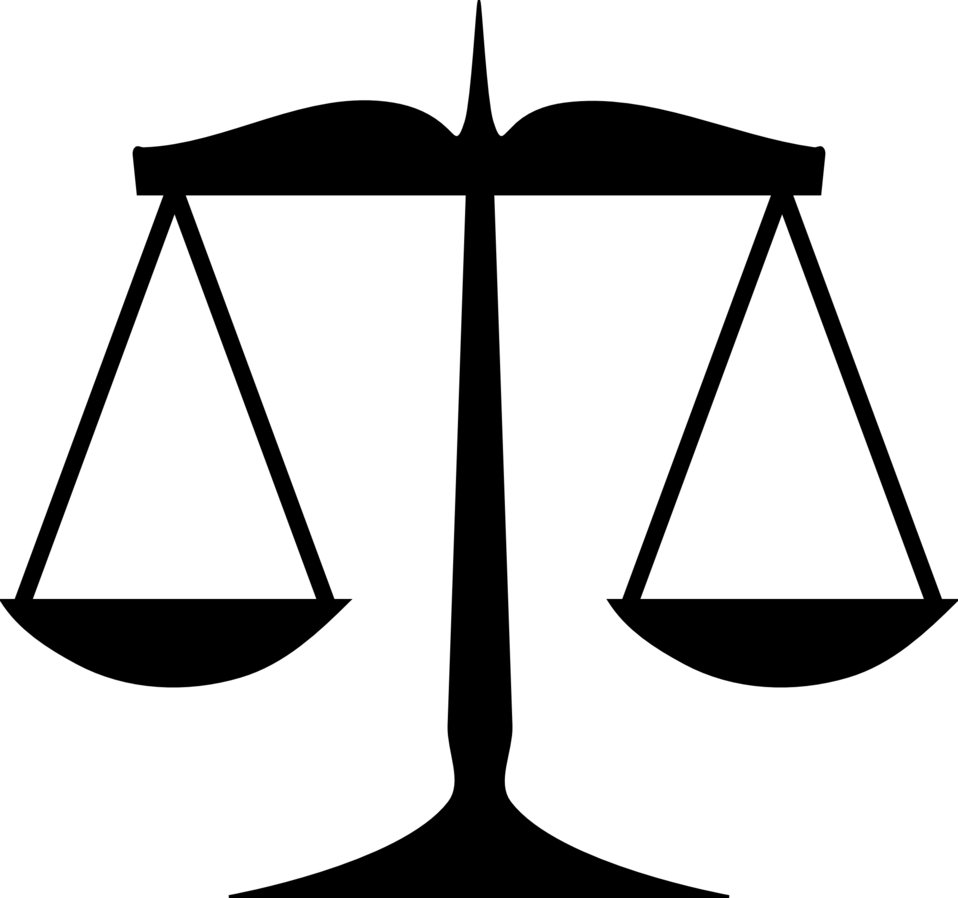
\includegraphics[scale=.2]{twoPanBalance}

  \textit{[In class we solved this using a numeric scale (e.g. a spring scale) that gives the exact weight
  of a pile of coins; our algorithm took $\ceil{log_2(n)}$ weighings in the worst case. Using a two-pan balance
  scale you can do better!]}

  \item Generalize the algorithm from part a: How do you find the fake coin if there are $n$ coins
  (for some $n \geq 1$)? How many weighings (as a function of $n$) does
  your algorithm require in the worst case?
\end{enumerate}

\medskip
\textbf{Problem 2: Multiplication}

Come up with an algorithm for multiplying two 6-digit numbers using as little multiplication as possible:
You can only directly multiply 3-digit numbers (or smaller), and you can only do at most 4 such multiplications.
Inserting/removing trailing 0s (i.e. multiplying or dividing by powers of 10) doesn't count against your limit of 4,
and you are also allowed to use 3 additions.

\textit{[Where do these strange restrictions come from? Computers are faster at addition and at inserting/removing trailing
0s than they are at multiplication, so this problem simulates how computers actually multiply very large numbers
using a divide-and-conquer algorithm. The actual algorithm uses only 3 multiplications rather than 4 - if you want
an extreme challenge you can try to come up with that one!]}

\medskip
\textbf{Problem 3: Coin Removal}

There is a line of $n$ coins on the table; some of them are heads up and the rest are tails up, in no particular
order. The object of the puzzle is to remove all the coins by a sequence of moves. On each move, one can
remove any head-up coin, after which its neighboring coin or coins, if any, must be turned over. Coins are
considered ``neighbors'' only if they are next to each other in the original line; coins that have a gap between them
(because the coins originally in that gap have been removed) are not considered neighbors.
Determine the property of the starting line that is necessary and sufficient for the puzzle to have a
solution. For those lines that can be removed by the puzzle's rules, design an algorithm for doing so.

\end{document}
